\chapter{Implementace}

Tato kapitola popisuje implementaci řešení. V první části je popsán vývoj klientské a serverové části webové aplikace včetně API, následující části se 
věnují implementaci Plánovače a kontejnerizaci.

\section{Webová aplikace}

Vývoj webové aplikace probíhal v iteracích, během kterých byly postupně implementovány jednotlivé funkce. Zástupci organizátorů akce SummerJob
měli k aplikaci přístup od začátku vývoje, což umožnilo průběžné testování a získávání zpětné vazby. Aplikace byla během vývoje dostupná na dočasné webové adrese.

Vybraný framework Next.js využívá rozšířenou verzi technologie React pro implementaci klientské části.
Od verze 13 podporuje Next.js experimentálně kompletní či částečné renderování na straně serveru, které je využíváno pro optimalizaci výkonu a přenesených dat.
Částečná tvorba výsledných stránek na serveru umožňuje využít přístup k databázi bez nutnosti následných požadavků na API, což snižuje dobu načítání stránky.
Také je možné využít statické generování, které je vhodné pro neměnná data, například chybové stránky. Stránka je během sestavení aplikace vygenerována a v případě chyby
je klientské části předána jako statický obsah. Výhodou je rychlejší zobrazení oproti vykreslování pomocí JavaScriptu na straně klienta a menší zatížení serveru, než v případě
dynamického serverového renderování. Výsledná aplikace je tedy kombinací statických a dynamických stránek. Vzhledem k výhodám tohoto přístupu byla zvolena verze 13 frameworku Next.js
i přes experimentální verzi. Tým Next.js aktivně vyvíjí a testuje nové verze a experimentální funkce jsou stabilní a bezpečné. S ohledem na historii
vývoje frameworku a jeho popularitu je pravděpodobné, že bude stabilní verze vydána průběhu tohoto roku \cite{nextjs_versions}.

\subsection{Klientská a serverová část}

Vybraný framework Next.js využívá technologii React pro implementaci klientské části. React je knihovna pro tvorbu uživatelských rozhraní, která je vyvíjena
společností Facebook \cite{react}. Využívá komponentovou architekturu, která umožňuje znovupoužitelnost a zapouzdření kódu. Komponenty jsou nezávislé na sobě a
komunikují pomocí vstupních a výstupních parametrů. Výstupem komponenty je virtuální DOM, který je následně porovnán s aktuálním DOM a provedeny
pouze změny, které jsou nutné. Tento přístup umožňuje efektivní aktualizaci uživatelského rozhraní a zajišťuje vysoký výkon aplikace. React je
vyvíjen jako open-source projekt a je využíván v mnoha projektech, například v aplikaci Facebook, Instagram, Netflix a dalších \cite{react_used}.

Pro zápis kódu využívá React rozšíření jazyka JavaScript, které se nazývá JSX. JSX umožňuje vkládat HTML kód přímo do JavaScriptu, což má za cíl
zjednodušit tvorbu uživatelského rozhraní. Podporuje i TypeScript ve formátu TSX, který dále rozšiřuje JSX o typové informace.
Výhodou je kontrola syntaxe a typů při kompilaci, což umožňuje odhalit chyby v kódu před spuštěním aplikace. Ukázka kódu \ref{code:jsx} zobrazuje
komponentu, která je zobrazena brigádníkům, pokud na daný den nejsou přiřazeni k žádné práci.

\begin{listing}[h]
  \begin{minted}{jsx}
export default function MyPlanEmpty() {
  return (
    <>
      <PageHeader title={"Můj plán"} isFluid={false} />
      <section>
        <div className="container">
          <Box>
            <h5>Nemáte naplánované žádné činnosti.</h5>
          </Box>
        </div>
      </section>
    </>
  );
}
    \end{minted}
    \caption{Ukázka kódu v TSX pro zobrazení prázdného plánu}
    \label{code:jsx}
\end{listing}

Next.js podporuje tvorbu serverové části aplikace, která je v aplikaci využita pro správu dat a tvorbu API. 
Struktura cesty, na které se konkrétní stránky zobrazují, je definována pomocí umístění souboru v adresáři \texttt{app}.
Soubor \path{app/admin/logs/page.tsx} se tedy zobrazí na adrese \path{example.com/admin/logs/page}.
Pro dynamické segmenty cesty je možné využít hranaté závorky, například \path{app/admin/[id]/page.tsx}. Komponenta v daném souboru
v tomto případě jako parametr přijímá objekt \texttt{params}, který obsahuje hodnoty dynamických segmentů cesty.
Stránky je také možné seskupovat do transparentních skupin, které se neprojeví v URL adrese, pomocí kulatých závorek. V aplikaci se toto oddělení využívá 
například pro skupinu stránek určených k tisku dokumentů. Stránka pro tisk dokumentu, definovaná v souboru \path{app/(print)/print-plan/page.tsx}, se 
zobrazí na adrese \path{example.com/print-plan}.

Operace s daty a ověřování správnosti
dat je nutné provádět na serveru, aby bylo zajištěno, že data v databázi jsou vždy logicky validní. Aplikace tak například neumožní vytvoření
dvou aktivních událostí zároveň nebo přiřazení pracanta k více pracím současně.
Serverová část je implementována pomocí Node.js a využívá TypeScript, který je před spuštěním aplikace kompilován do JavaScriptu.


\subsection{Přihlašování}

Správa přihlašování je implementována pomocí knihovny NextAuth.js. Knihovna podporuje
přihlašování pomocí e-mailu, služeb Google, Facebook, GitHub, Twitter, Apple a dalších \cite{nextauth}. Přihlašování pomocí uživatelského jména a hesla je autory knihovny 
považováno za nebezpečné a pro podporu je nutné implementovat vlastní ověření uživatelů. Na základě analýzy bylo proto zvoleno přihlašování pomocí e-mailu.
K odesílání e-mailů využívá NextAuth.js balíček \texttt{nodemailer}, který umožňuje odesílání e-mailů pomocí protokolu SMTP. Pro odesílání e-mailů je nutné
zvolit poskytovatele SMTP služby, vlastní e-mailový server není součástí řešení. Vzhled a obsah e-mailů je možné upravit pomocí šablon, které jsou součástí
implementace.

Přihlašování je první částí aplikace, která se zobrazí nepřihlášenému uživateli. Pokus o přístup na stránku, která vyžaduje přihlášení,
je zachycen na straně serveru a uživatel je přesměrován na přihlašovací stránku. Nedochází tedy k úniku citlivých dat nebo jiného interního obsahu.

Přihlašovací stránka obsahuje formulář s polem pro zadání e-mailové adresy. Po odeslání formuláře dojde k ověření existence uživatele v databázi.
Pokud je uživatel registrovaný v aktuálním ročníku akce a nejedná se o blokovaný účet, je uživateli odeslán e-mail s odkazem pro přihlášení a na stránce je 
zobrazena příslušná informace. Pokud uživatel neexistuje nebo je jeho účet blokovaný, je zobrazena chybová hláška.

Přihlášení pomocí odkazu v e-mailu je zabezpečeno pomocí jednorázového tokenu s omezenou časovou platností, který je generován při odeslání e-mailu.
Po přihlášení je token z databáze odstraněn.
Webovému prohlížeči je přiřazeno identifikační cookie s platností jeden měsíc, které je využíváno pro autentizaci uživatele. Během této doby se uživatel nemusí v
daném prohlížeči znovu přihlašovat. Platnost po dobu jednoho měsíce byla zvolena s ohledem na dobu trvání akce SummerJob -- jedná se o přípravu na ročník,
týden práce a čas pro vyřízení administrativy po skončení akce.

Ověřování dotazů na server probíhá pomocí knihovny NextAuth.js, která využívá databázi pro ukládání uživatelů a jejich identifikačních údajů. Při každém přechodu na stránku
nebo dotazu na API je na server odeslán požadavek s cookie, která obsahuje identifikátor relace. Server ověří platnost relace v databázi a v případě úspěchu jsou zobrazeny
požadované údaje. V případě neplatného identifikátoru je uživatel přesměrován na přihlašovací stránku. Knihovna NextAuth.js umožňuje také správu přihlášení bez použití databáze pomocí
technologie JWT\footnote{JSON Web Token}, která umožňuje ověření uživatele pomocí serverem šifrovaného tokenu. Token obsahuje informace o uživateli 
a při každém požadavku dochází k jeho ověření na serveru bez nutnosti přístupu k databázi. Tento způsob však neumožňuje snadno zneplatnit relaci uživatele, například při změně aktivního ročníku.
Také není vhodný pro informace, které se mohou v čase měnit, například oprávnění uživatele. Proto byla zvolena strategie ověřování pomocí databáze.

Cookie využívá atributy \texttt{HttpOnly} a \texttt{SameSite}, které zabraňují přístupu k hodnotě cookie ze skriptů a
pomáhají předcházet útokům typu CSRF. Dále je cookie chráněno proti úniku přes nezabezpečené připojení pomocí atributu \texttt{Secure}. 

Registrace dobrovolníků je řešena externě a organizátoři mají možnost importovat seznam vybraných dobrovolníků do databáze v záložce \textit{Pracanti}.

\subsection{Oprávnění}

Uživatelé byli rozděleni do několika skupin podle požadovaných oprávnění. Každá skupina má přístup k jiným částem aplikace, které jsou pro ni relevantní.
Je tak možné určit organizátory, kteří mají přístup k evidenci dobrovolníků, skupinu zodpovědnou za tvorbu plánů, administrátory a další.
Oprávnění byla rozdělena do následujících skupin:

\begin{itemize}
    \item \textbf{Admin:} administrátoři mají přístup ke všem částem aplikace. Jsou oprávnění měnit nastavení ročníku, přidávat nové ročníky, určovat oprávnění jiných uživatelů, zablokovat přihlášení uživatele a další.
    \item \textbf{Plány:} uživatelé s oprávněním \textit{Plány} mají přístup k tvorbě plánů a jejich úpravě. Pro tento účel mají pomocí API přístup k evidenci dobrovolníků, aut i prací, ale nemohou je upravovat.
    \item \textbf{Pracanti:} uživatelé s oprávněním \textit{Pracanti} mají přístup k evidenci dobrovolníků. Můžou do ní přidávat nové záznamy, upravovat je a mazat.
    \item \textbf{Auta:} uživatelé s oprávněním \textit{Auta} mají přístup k evidenci aut. Auta lze přidávat, upravovat a odstraňovat. Pro přiřazení auta k majiteli mají pomocí API přístup k evidenci dobrovolníků, ale nemohou ji upravovat.
    \item \textbf{Práce:} oprávnění \textit{Práce} umožňuje přidávat, upravovat a mazat navrhované práce. Toto oprávnění neumožňuje měnit naplánované práce.
\end{itemize}

Kontrola oprávnění přístupu na webovou stránku probíhá na serveru. Na základě relace přihlášeného uživatele je vyhodnoceno, zda má přístup k požadované stránce.
V případě, že uživatel nemá oprávnění, je uživateli zobrazena chybová stránka s informací o nedostatečných oprávněních.
Oprávnění je kontrolováno v souborech \texttt{layout.tsx}, které slouží jako kořenové šablony pro skupiny stránek. Kód v souboru se vykoná před vykreslením
jiných stránek ze skupiny a slouží k sestavení základního vzhledu stránky společného pro všechny stránky ve skupině, do kterého je na určené místo vložena konkrétní stránka.
Je tak možné například jednotně definovat vložení záhlaví stránky, které obsahuje navigační menu a tlačítko pro odhlášení. Šablony je možné vnořovat.
V ukázce \ref{code:cars-layout} je soubor \texttt{layout.tsx} pro skupinu stránek \textit{Auta}, který kontroluje, zda má uživatel požadované oprávnění.
Administrátorská práva není nutné při kontrole specifikovat, protože administrátoři mají přístup ke všem stránkám.

\begin{listing}[h]
  \begin{minted}{jsx}
export default async function CarsLayout({children}: {
  children: React.ReactNode;
}) {
  const permsCheck = await withPermissions([Permission.CARS]);
  if (!permsCheck.success) {
    return <AccessDeniedPage />;
  }
  return <>{children}</>;
}
    \end{minted}
    \caption{Kontrola oprávnění pro přístup ke stránkám ve skupině Auta}
    \label{code:cars-layout}
\end{listing}

\subsection{Získávání dat}

Data jsou získávána pomocí API, které je popsáno v samostatné kapitole. Pro komunikaci s API byla využita knihovna \texttt{SWR} od vývojářů Next.js, která
rozšiřuje funkce standardní knihovny \texttt{fetch} a je vhodná pro použití v React aplikacích. Knihovna je založena na principu \textit{stale-while-revalidate},
který zajišťuje plynulou aktualizaci dat. Při prvním načtení dat je zobrazena poslední stažená verze a následně jsou data aktualizována na pozadí. Tento přístup
umožňuje rychlé zobrazení dat i v případě pomalého připojení, pokud jsou data již stažena a uložena v prohlížeči. Lze nastavit automatickou aktualizaci dat 
v pravidelných intervalech, což je využito například při zobrazení aktuálního stavu plánů. Ve výchozím nastavení nestahuje data, pokud daná karta prohlížeče není
aktivní, což šetří přenosové pásmo a zdroje serveru. Umožňuje také deduplikovat data, pokud je více požadavků na stejnou URL.

Pokud dojde k chybě při získávání dat, SWR se pokusí požadavek zopakovat. Během této doby jsou zobrazena data z cache, pokud jsou k dispozici. Tento způsob
umožňuje zobrazovat data i při přerušení připojení k internetu. Po obnovení spojení dojde k automatické aktualizaci dat a zobrazení nových hodnot.

Knihovna umožňuje provádět i jednorázové požadavky, které nejsou ukládány do cache. Tento přístup se využívá pro vytváření, úpravu a mazání dat, kdy není vhodné
opakovat požadavky na server.

Pro zrychlení načítání dat aplikace využívá předání serializovaných dat přímo ze serveru během server side renderingu. Tento přístup je využit například při
zobrazení seznamu prací -- data jsou na serveru načtena z databáze, serializována, předána do React aplikace a odeslána klientovi.
Data jsou v prohlížeči deserializována spolu se strukturou stránky a zobrazena, následně jsou aktualizována pomocí SWR na pozadí. Tento přístup umožňuje zobrazit data okamžitě, aniž by
uživatel musel čekat na jejich stažení po načtení skriptů, které následně načítají data z API.
Nedochází tak například k zobrazení prázdné tabulky a následnému překreslení po stažení dat.

\subsection{Rozvržení aplikace}

Klientská část webové aplikace je rozdělena do několika částí, které jsou popsány níže. Každá část je zobrazena v samostatné záložce, která je přístupná
pouze s odpovídajícím oprávněním. Všechny záložky jsou dostupné z hlavního menu, které je zobrazeno v horní části obrazovky.

Pro zobrazení evidencí byly zvoleny tabulky, které jsou vhodné pro zobrazení strukturovaných dat v horizontálních řádcích.
Během plánování je nutné přehledně zobrazit velké množství dat, například informace o práci, brigádnících a autech pro každou naplánovanou práci.
Na mobilních zařízeních s vertikálně orientovaným displejem však nebylo možné efektivně zobrazit všechny potřebné informace.
Řazení všech informací pod sebe by vedlo k přílišnému prodloužení stránky a ztížilo by to orientaci v datech. Po konzultaci s organizátory
bylo rozhodnuto o zobrazení dat v posuvných tabulkách. Nevýhoda tohoto řešení je však v tom, že na mobilních zařízeních není možné zobrazit všechny
informace najednou. Uživatel musí horizontálně posouvat tabulku, aby zobrazil všechny sloupce. Toto řešení bylo zvoleno jako kompromis mezi
přehledností a přístupností. Plánování a náročné operace jsou prováděny převážně na počítačích, kde je dostatek místa pro zobrazení všech informací,
zatímco mobilní rozhraní slouží převážně pro jednorázové změny. Srovnání zobrazení dat na počítači a mobilním zařízení je zobrazeno na obrázcích \ref{fig:plan-pc} a \ref{fig:plan-mobile}.

\begin{figure}[ht]
    \centering
    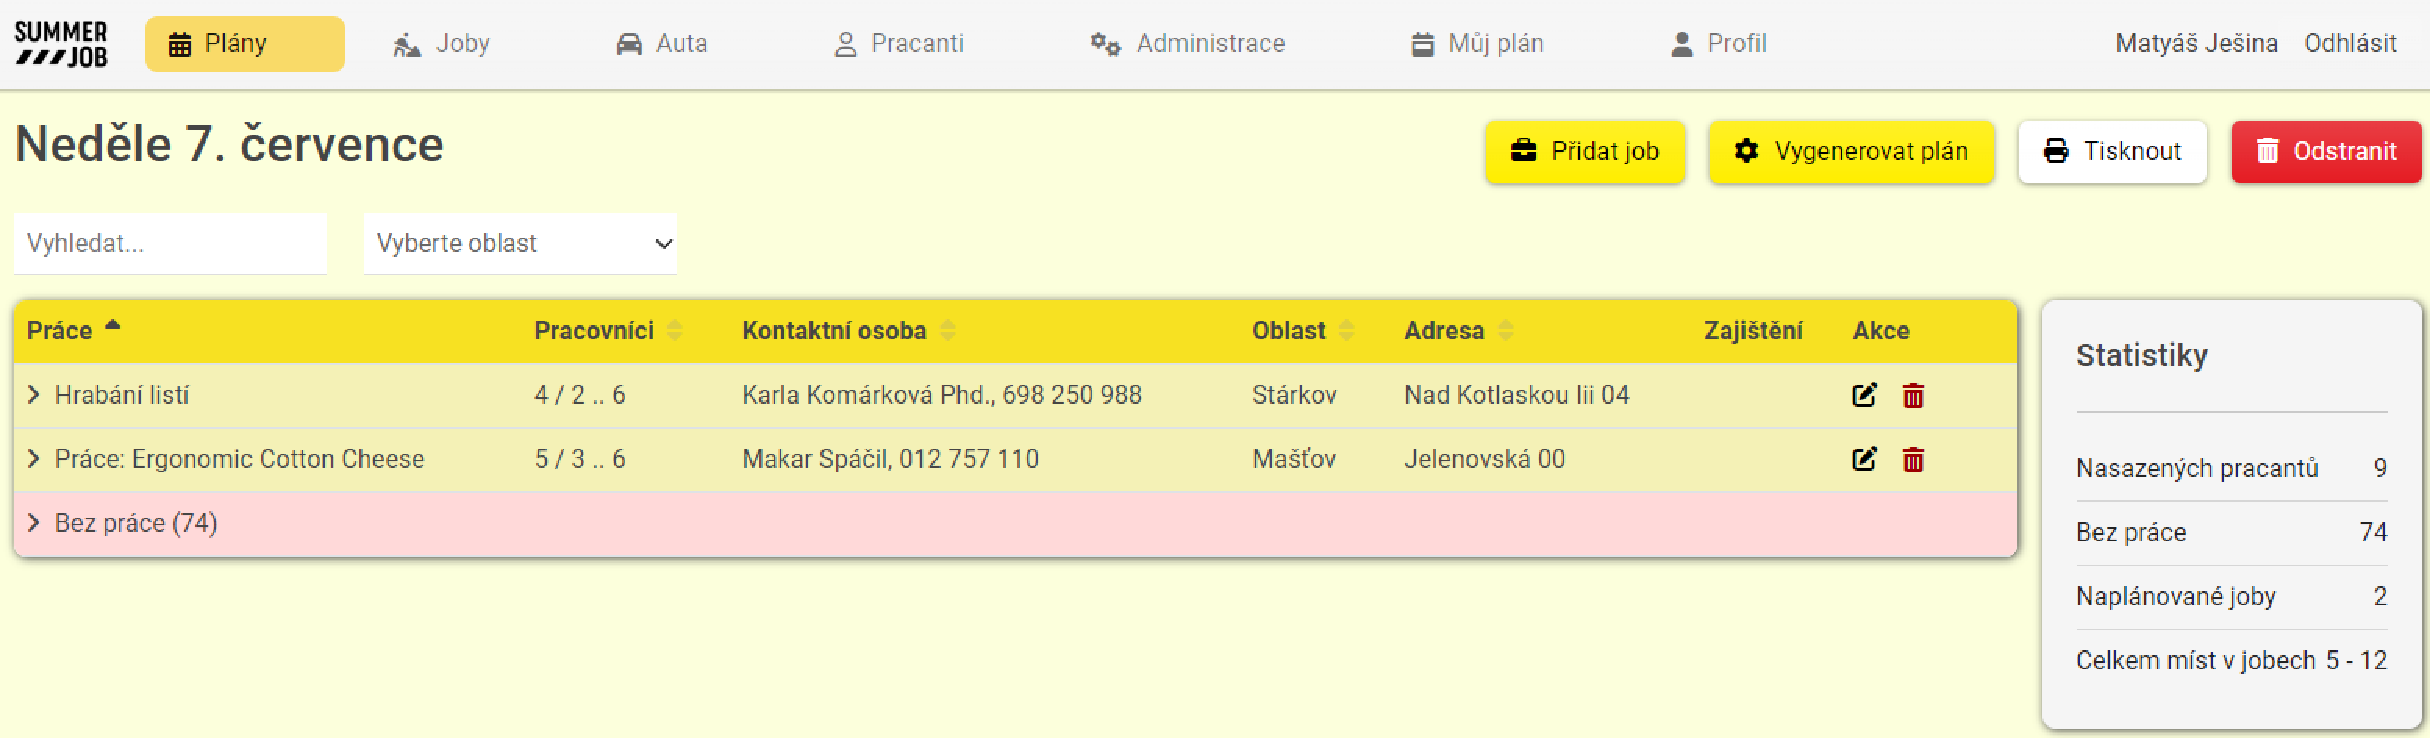
\includegraphics[width=0.9\textwidth]{chapters/images/plan-pc.pdf}
    \caption{Zobrazení tabulky s plánem na počítači}
    \label{fig:plan-pc}
\end{figure}

\begin{figure}[ht]
    \centering
    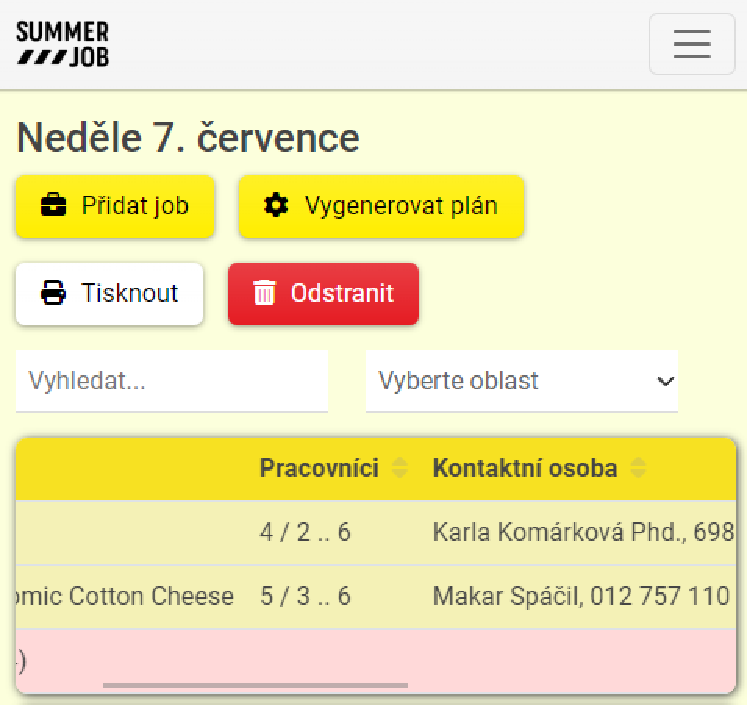
\includegraphics[width=0.9\textwidth]{chapters/images/plan-mobile.pdf}
    \caption{Zobrazení tabulky s plánem na mobilním zařízení}
    \label{fig:plan-mobile}
\end{figure}


\subsubsection{Pracanti}

Záložka \textit{Pracanti} obsahuje seznam registrovaných brigádníků. Seznam je zobrazen v tabulce, která umožňuje vyhledávání a filtrování dat.
Jsou zde zobrazeni pouze brigádníci, kteří jsou registrovaní v aktuálním ročníku akce. U každého brigádníka je zobrazeno jméno, e-mail, telefonní číslo,
e-mailová adresa a speciální vlastnosti. Tyto vlastnosti v současnosti zahrnují informaci o tom, zda má brigádník k dispozici auto a zda je brigádník silný,
což je důležité pro plánování prací.

U každého pracanta jsou dále evidovány alergie a dny, kdy může pracovat. Tyto informace je možné zobrazit a upravit na samostatné stránce, která je dostupná
po kliknutí na ikonu úprav v příslušném řádku tabulky. Na této stránce je také možné zobrazit a upravit přihlašovací údaje brigádníka. Pro zobrazení a úpravu
pracantů je nutné mít příslušná práva, bez kterých není možné ani přistoupit na stránku.

Stránka umožňuje také přidávat nového brigádníka do databáze. Přidání nového brigádníka je řešeno pomocí formuláře, který obsahuje pole pro všechny evidované
hodnoty. V případě neplatného vstupu je uživatel upozorněn chybovou hláškou. Validace je řešena na straně klienta pomocí knihovny Zod, která umožňuje definovat
schéma dat a následně je použít pro validaci vstupu. Validace je také řešena na straně serveru stejným způsobem. Kromě individuálního přidávání je možné využít
funkci pro hromadný import, která umožňuje vložení seznamu brigádníků a jejich údajů ve formátu dat oddělených středníkem. Uživateli je před odesláním
k dispozici náhled importovaných dat.

Na žádost organizátorů byla do aplikace přidána možnost tisku seznamu brigádníků v jednoduché tabulce. Tato funkce je dostupná v záložce \textit{Pracanti} po kliknutí
na tlačítko \textit{Tisknout}.

\subsubsection{Joby}

V záložce \textit{Joby} jsou zobrazeny všechny práce, které je možné vykonat během akce. U každé práce je evidován název, popis, minimální
a maximální počet brigádníků, kteří mohou danou práci vykonávat současně, a počet silných brigádníků, kteří jsou pro práci potřeba. Dále jsou evidovány
informace o lokalitě, kde se práce bude vykonávat, včetně přesné adresy, kontakt na zadavatele, počet dnů potřebných pro vykonání práce, 
seznam dní, kdy je možné práci vykonávat, a alergeny v místě pracoviště. Evidence alergenů umožní automatickému plánovači i organizátorům přiřadit na práci brigádníky, kteří nemají
konfliktní alergie s alergeny na pracovišti. Data obsahují také údaj, zda je v místě práce dostupná sprcha a občerstvení. 
U jobu je možné zadat soukromou a veřejnou poznámka. Veřejná poznámka slouží jako popis práce, který je po naplánování
zobrazen brigádníkům. Soukromá poznámka je určena pouze pro organizátory a slouží k interní komunikaci. Evidované joby slouží jako předloha pro práce přidávané
do plánu. Tento typ jobů je v aplikaci interně označen jako \textit{Proposed Job}, neboli navrhovaná práce, která ale nemusí být naplánována.

Do seznamu je možné přidávat nové práce a upravovat již existující, vyhledávat a filtrovat.
Jednotlivé joby je možné označit jako splněné nebo nežádoucí, což umožňuje organizátorům filtrovat práce, které již nejsou potřeba. Takové práce jsou v seznamu
zařazeny na konec stránky. Připnutí naopak umožňuje organizátorům označit práci jako důležitou a zobrazit ji na začátku seznamu. Označené joby jsou od standardních
barevně odlišeny.

\subsubsection{Auta}

Záložka \textit{Auta} obsahuje seznam aut, která jsou k dispozici pro přepravu brigádníků na pracoviště. U každého auta je evidován název, počet míst, majitel,
najeté kilometry a poznámka. Majitelem je vždy některý z registrovaných brigádníků. Na stránce je možné přidat, upravovat a odebírat auta.

Pro vyplacení kompenzace za použití auta je nutné evidovat počet najetých kilometrů. Na začátku je do systému zaznamenán stav odometru a po skončení akce
se na základě tohoto údaje a aktuálního stavu odometru vypočítá počet najetých kilometrů. Tato hodnota je následně použita pro výpočet kompenzace. Aplikace 
umožňuje evidovat výši kompenzace a údaj, zda došlo k proplacení.

\subsubsection{Plány}

Záložka \textit{Plány} obsahuje seznam plánů, které byly vytvořeny pro aktuální ročník akce. Na každý den akce vzniká nový plán, který zahrnuje
seznam brigádníků a jejich přiřazení na práce.

Plán je možné vytvořit ručně nebo automaticky. Ruční vytvoření plánu je řešeno pomocí formuláře, který umožňuje vybrat práce pro daný den a následně 
k nim přiřadit brigádníky. Organizátoři mohou naplánovat dopravu na pracoviště, systém umožňuje také sdílet dopravu s jinou prací. K vytvořenému záznamu
o práci je možné přidávat poznámky. Z přiřazených brigádníků je vybrána zodpovědná osoba, která zodpovídá za komunikaci s organizátory a zadavatelem a za správné vykonání práce.
Práce přiřazené v plánu jsou v aplikaci interně označeny jako \textit{Active Job}, neboli aktivně naplánovaná práce. Každá aktivní práce má předlohu v evidenci jobů.
K práci je možné přiřadit soukromý a veřejný popis, které jsou ve výchozím nastavení shodné s popisem předlohy. Soukromý popis slouží k interní komunikaci organizátorů,
veřejný popis je zobrazen brigádníkům v plánu.

Plánování je klíčovou součástí aplikace a musí být jednoduché a intuitivní. Naplánované práce jsou zobrazeny v tabulce, řádky obsahují
základní informace o práci, jako je název, počet brigádníků nebo lokalita. Podrobné informace je možné zobrazit kliknutím na řádek. Po kliknutí 
dojde k rozbalení řádku a zobrazení podrobností o práci, jako je popis, jména brigádníků, zodpovědná osoba, seznam dopravy a poznámka pro organizátory.
Seznam pracantů je možné upravovat pomocí tlačítka vedle jména jednotlivých brigádníků nebo pomocí přetáhnutí řádku se jménem pracanta do jiné práce.
Stejným způsobem lze přiřazovat i zatím nepřiřazené brigádníky. V seznamu jízd u dané práce se zobrazují pouze jízdy řidičů, kteří jsou přiřazeni na danou práci.
Pokud je do jízdy zařazen brigádník z jiné práce, je jeho jméno uvedeno u příslušného záznamu. Ukázka je k dispozici na obrázku \ref{fig:plan-expanded}.

\begin{figure}[h]
    \centering
    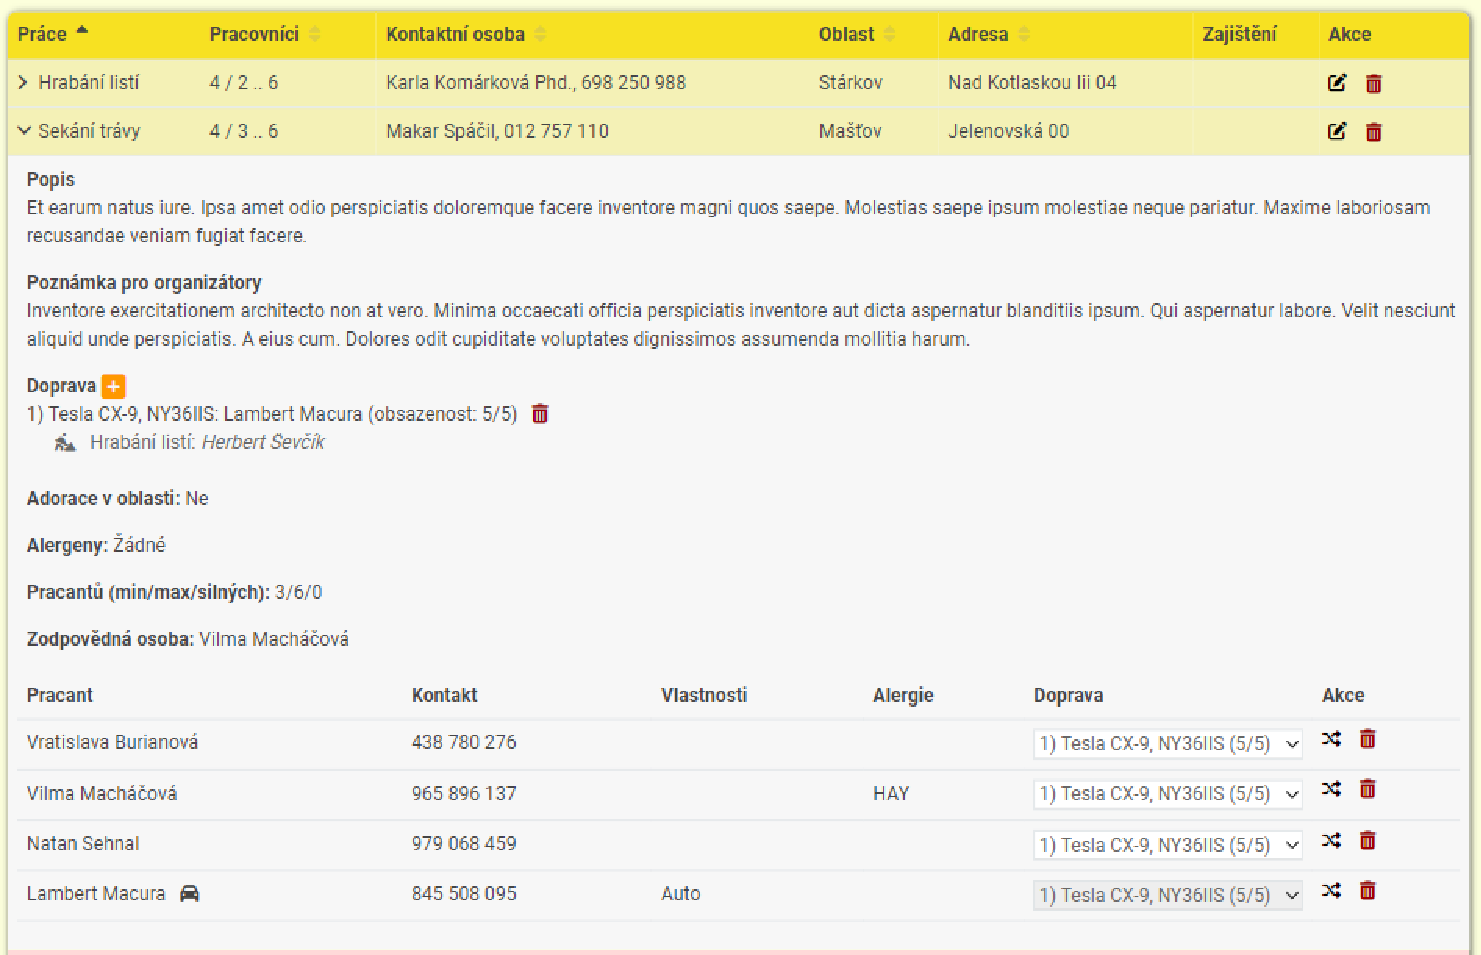
\includegraphics[width=0.9\textwidth]{chapters/images/plan-expanded.pdf}
    \caption{Rozbalený řádek s prací v plánu}
    \label{fig:plan-expanded}
\end{figure}


Aplikace automaticky rozpoznává konflikty v plánu a upozorní organizátory pomocí varovného symbolu v řádku tabulky a popisu konfliktu.
Konflikty mohou vzniknout v případě, že je na práci přiřazen nedostatek nebo přebytek brigádníků, 
chybí doprava, není přiřazena zodpovědná osoba, je přiřazen pracovník s konfliktní alergií, nebo je přiřazen pracovník, který projevil zájem o adoraci v daný den,
ale v dané lokalitě není možné požadavek splnit.

Stránka s plánem zobrazuje také statistiky pro daný den. Jsou zde zobrazeny informace o počtu brigádníků, kteří jsou přiřazeni na práci, počtu brigádníků, kteří
práci nemají, počet prací v plánu a rozsah počtu pracovníků, které lze daný den na vybrané práce přiřadit.

Je zde možnost využít automatické plánování, řešené pomocí algoritmu, který je popsán v kapitole \ref{sec:planner}. Po výběru prací na daný den a spuštění
plánovače dojde k automatickému přiřazení brigádníků na práce tak, aby nebyl vytvořen žádný konflikt. Pokud je v plánu již nějaký brigádník přiřazen na práci, 
plánovač přiřazení zachová. Dojde také k naplánování dopravy a přiřazení zodpovědné osoby. Pokud není možné vytvořit plán bez konfliktů, 
vytvoří plánovač plán blízký optimálnímu řešení. Veškeré konflikty jsou zobrazeny v seznamu na stránce plánu.

Plánování podporuje práci více uživatelů současně. Během plánování dochází na pozadí k pravidelné aktualizaci dat, aby bylo zajištěno,
že uživatelé pracují s nejnovější verzí plánu. K aktualizaci dochází v intervalu 1 sekundy a k přenosu dat dojde pouze tehdy, pokud došlo od posledního požadavku ke změně,
čímž je minimalizován počet přenesených dat.

Aplikace umožňuje zobrazit plán v tisknutelné podobě. Jedná se o zjednodušenou černobílou verzi plánu v kompaktním zobrazení, které je vhodné pro tisk na 
papír velikosti A4. Dodatečné CSS styly zajišťují správné rozdělení plánu na papír tak, aby naplánovaná práce nepřesahovala na více stran současně.

\subsubsection{Administrace}

Záložka \textit{Administrace} slouží k nastavení aktuálního ročníku a oblastí, ve kterých se akce koná. Aktivní ročník
označuje právě probíhající akci a eviduje datum začátku a konce akce. Ve správě ročníku je možné upravovat informace o oblastech, ve kterých
se ročník koná. Atributy oblastí zahrnují název oblasti, nutnost dopravy a možnost adorace. Maximálně jeden ročník může být označen jako
aktivní současně, ostatní ročníky jsou automaticky deaktivovány při aktivaci nového ročníku. Při deaktivaci dochází automaticky 
k odhlášení všech přihlášených uživatelů bez administrátorského oprávnění a zablokování opětovného přihlášení.

Jednotlivé uživatelské účty je možné zablokovat nebo odblokovat z administračního rozhraní i v průběhu ročníku. Účastník se zablokovaným účtem
se nemůže přihlásit do systému, ale jeho údaje zůstávají zachovány a je možné s uživatelem dále pracovat. Administrátor také může uživatelům
přiřazovat a odebírat oprávnění.

V této části aplikace také možné prohlížet záznamy o změnách v systému, tzv. \textit{audit log}. Záznamy zahrnují veškeré akce, které mění data v databázi,
například vytvoření, úpravu nebo smazání záznamu. Záznamy jsou řazeny chronologicky a obsahují informace o uživateli, který změnu provedl,
o čase změny a o změněných datech. V záznamech je možné vyhledávat a filtrovat podle typu události.

\subsubsection{Můj plán}

Záložka \textit{Můj plán} zobrazuje seznam prací, na které je uživatel přiřazen. Brigádník může zobrazit detail práce pro daný den,
který obsahuje informace místě a popis práce, jména dalších brigádníků přiřazených na práci a způsob dopravy.

\subsubsection{Profil}

Záložka \textit{Profil} zobrazuje informace o uživateli. Uživatel může upravit své osobní údaje, označit dny, kdy může pracovat a adorovat,
a nastavit své případné alergie.

\section{API}

Pro implementaci API bylo využito Next.js API Routes. Jedná se o speciální stránky Next.js, které jsou přístupné na URL \textit{/api/*} a slouží k implementaci API.
Ve složce projektu jsou tyto soubory uloženy ve složce \textit{pages/api}.
API dodržuje REST architekturu a využívá HTTP metody pro komunikaci. Pro přístup a úpravu dat je nezbytná autorizace pomocí session cookie, která je zaslána v hlavičce HTTP požadavku.

V době psaní práce dochází k přepracování původních API Routes na novou verzi. Nová verze API bude přesunuta do složky \textit{app/api} a nabízí automatické volání
funkcí pro příslušné HTTP metody. Porovnání původního a nového způsobu zápisu API je uveden v ukázkách kódu \ref{code:api-old} a \ref{code:api-new}.
Implementace využívá původní způsob zápisu API z důvodu lepší kompatibility s existujícími nástroji a knihovnou NextAuth. Podle autorů Next.js budou oba způsoby zápisu API
podporovány i v dalších verzích. Nová verze API nepřináší oproti použité implementaci významné výhody.

\begin{listing}[h]
  \begin{minted}{typescript}
export default async function handler(
  req: NextApiRequest,
  res: NextApiResponse
) {
  if (req.method === "GET") {
    // handle GET request
    return res.status(200).json({ data });
  } else if (req.method === "POST") {
    // handle POST request
  } else {
    res.status(405).end();
  }
}
  \end{minted}
  \caption{Původní způsob zápisu API}
  \label{code:api-old}
\end{listing}

\begin{listing}[h]
\begin{minted}{typescript}
export async function GET(request: Request) {
  // handle GET request
  return NextResponse.json({ data })
}

export async function POST(request: Request) {
  // handle POST request
}
  \end{minted}
  \caption{Nový způsob zápisu API}
  \label{code:api-new}
\end{listing}

\subsection{Způsob komunikace}


Pro komunikaci s API byla zvolena REST\footnote{REST, Representational State Transfer} architektura, což je architektura webových služeb používaná pro výměnu dat mezi klientem a serverem \cite{rest}. REST API se vyznačuje následujícími charakteristikami:

\begin{itemize}
  \item \textbf{Klient-server architektura:} klient a server jsou odděleni.
  \item \textbf{Bezstavovost:} každý požadavek klienta obsahuje všechny informace, které server potřebuje pro vyřízení požadavku, bez potřeby zachování stavu mezi požadavky.
  \item \textbf{Jednotné rozhraní:} REST API poskytuje jednotné rozhraní pro přístup k různým zdrojům dat, které jsou identifikovány pomocí URL adresy.
\end{itemize}

REST API umožňuje vývojářům vytvářet aplikace, které mohou komunikovat se serverem a získávat nebo odesílat data.
Klient může posílat požadavky na server pomocí HTTP metod, jako jsou GET, POST, PUT, PATCH, DELETE a další
a server odpovídá pomocí odpovědí s kódem stavu HTTP. Data v implementaci jsou přenášena ve formátu JSON. Zvolené metody
určují účel požadavku a jeho dopad na zdroje na serveru. V aplikaci byly implementovány následující metody:

\begin{itemize}
  \item \textbf{GET:} metoda GET se používá pro získání dat z určitého zdroje na serveru. Tato metoda neprovádí žádné změny na serveru a odpověď serveru obsahuje požadovaná data.
  \item \textbf{POST:} metoda POST se používá pro odeslání nových dat na server. Tato metoda se v aplikaci používá k vytvoření nového zdroje.
  \item \textbf{PATCH:} metoda PATCH se používá pro aktualizaci části existujícího zdroje na serveru. Tato metoda umožňuje aktualizaci pouze určitých částí datového zdroje na serveru, zatímco ponechává ostatní části beze změn.
  \item \textbf{DELETE:} metoda DELETE se používá pro odstranění zdroje na serveru. Tato metoda nevratně odstraňuje zdroj a jeho obsah z serveru.
\end{itemize}

Metody GET, PATCH a DELETE jsou idempotentní. Idempotentní metody garantují stejný výsledek operace bez ohledu na počet dotazů. Je tedy možné opakovaně
zasílat stejný požadavek bez neočekávaného chování. Metoda POST není idempotentní, protože při opakovaném zaslání stejného požadavku může dojít k vytvoření duplicitního zdroje. 
Ostatní metody definované ve standardu REST nejsou implementovány. REST API je rozšířeným standardem pro webové služby a je podporován mnoha moderními programovacími jazyky a frameworky.

\subsection{Swagger}

Pro dokumentaci API byl využit nástroj Swagger. Swagger je open-source framework pro návrh, vytváření, dokumentaci a používání REST API \cite{swagger_ui}.
Swagger UI umožňuje vytvořit interaktivní dokumentaci API, která je přístupná na URL \textit{/swagger} v režimu vývoje. Dokumentace obsahuje seznam všech dostupných
API endpointů, jejich popis, parametry a návratové hodnoty. Pro každý endpoint je možné vyzkoušet jeho funkčnost přímo v dokumentaci.
Náhled dokumentace je zobrazen na obrázku \ref{fig:swagger}.
Aplikace ve vývojovém režimu také obsahuje endpoint pro získání OpenAPI specifikace \cite{openapi} ve formátu JSON na adrese \textit{/api/swagger.json}.

\begin{figure}[h]
    \centering
    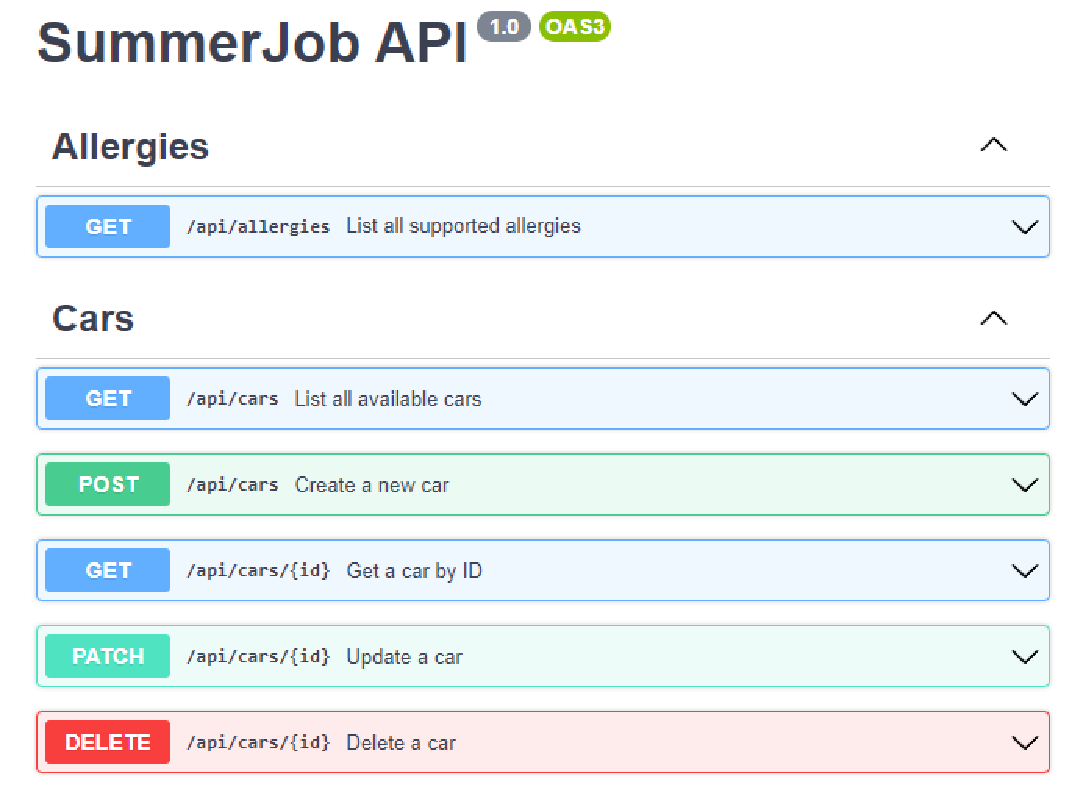
\includegraphics[width=1\textwidth]{chapters/images/swagger.pdf}
    \caption{Swagger dokumentace API}
    \label{fig:swagger}
\end{figure}

\subsection{Přihlášení}

Ověření uživatele není možné plně implementovat pomocí REST API, protože je nutné odeslat e-mail s přihlašovacím odkazem.
Je však možné přes API vyžádat odeslání e-mailu s přihlašovacím odkazem. Tento způsob využívá i webová aplikace, která při pokusu o přihlášení
vyžádá odeslání e-mailu a zobrazí uživateli další instrukce. Tento API endpoint spravuje knihovna NextAuth.js. Pro zvýšení bezpečnosti využívá knihovna
jednorázové CSRF tokeny. 

\subsection{Optimalizace}

Pro snížení objemu přenesených dat a zvýšení rychlosti odezvy API byly využity HTTP hlavičky \texttt{ETag}, \texttt{Last-Modified} a \texttt{If-None-Match}, které umožňují
posílat data pouze v případě, že jsou novější, než které má klient lokálně k dispozici.
Každý požadavek na API vrací v hlavičce ETag hash dat, která byla vrácena. Při dalším požadavku je možné v hlavičce If-None-Match poslat tento hash,
čímž se server rozhodne, zda vrátí data nebo pouze hlavičku s HTTP kódem 304 Not Modified. Tento způsob je využíván pro všechny požadavky, které vrací data.
Přenesená data jsou také komprimována pomocí gzip.

V případě opakovaných požadavků na stránce s plánem, které probíhají automaticky každou sekundu, se jedná o přenos přibližně 40 kB dat oproti
přibližně 5 MB za minutu, které by byly přeneseny bez využití těchto hlaviček. To umožňuje udržovat zobrazený plán stále aktuální i při pomalém či objemově limitovaném
připojení k internetu.

\subsection{Bezpečnost}

Aplikace využívá knihovnu Zod pro validaci dat \cite{zod}. Zod je knihovna pro TypeScript, která umožňuje definovat požadované typy a následně z těchto definic
vytvořit validátor, který ověří, zda vstupní data odpovídají definovaným typům. Validátory jsou vytvořeny pro všechna data, která jsou přijímána z API.
V případě, že data neodpovídají definovaným typům, dojde k odeslání HTTP kódu \texttt{400 Bad Request} s vysvětlením chyby.

Pomocí knihovny Zod je možné z validátorů automaticky vytvářet typy pro TypeScript a také ověřovat formuláře na straně klienta před odesláním.
To snižuje zátěž serveru kvůli kontrole neplatných vstupů a zároveň zvyšuje uživatelskou přívětivost.
Pro vytvoření Zod validačních schémat pro tabulky v databázi byl využit automatický generátor pro Prisma, který při změně datových typů v databázi
generuje validační schémata. Ukázka validačního schématu pro vytvoření uživatele je zobrazena v ukázce kódu \ref{code:zod}.
Zod umožňuje definovat i složitější valiátory, například pro pole objektů, nebo provádět operace s daty během validace.
V ukázce kódu je uveden validátor \mintinline{javascript}|z.date().or(z.string().min(1).pipe(z.coerce.date()))| -- tento typ umožňuje přijmout objekt typu \texttt{Date} nebo řetězec o minimální
délce~1, který lze převést na objekt typu \texttt{Date}. Pokud řetězec nelze převést na platné datum, dojde k chybě a validace se nezdaří.

\begin{listing}[h]
    \begin{minted}{javascript}
import { z } from "zod";

const WorkerCreateSchema = z
  .object({
    firstName: z.string().min(1),
    lastName: z.string().min(1),
    email: z.string().min(1).email(),
    phone: z.string().min(1),
    strong: z.boolean(),
    allergyIds: z.array(z.nativeEnum(Allergy)),
    availability: z.object({
      workDays: z
        .array(
            z.date().or(z.string().min(1).pipe(z.coerce.date()))
            )
      adorationDays: z
        .array(
            z.date().or(z.string().min(1).pipe(z.coerce.date()))
            )
    }),
  })
  .strict();
    \end{minted}
    \caption{Ukázka Zod validačního schématu pro vytvoření uživatele}
    \label{code:zod}
\end{listing}

Všechny požadavky na API kromě požadavků na přihlášení a čtení jsou zaznamenávány do databáze. Záznamy obsahují informace o uživateli, který požadavek
provedl, o čase požadavku, o cíli požadavku a zaslaná data. Tyto záznamy lze zobrazit v administračním rozhraní webové aplikace a jsou pouze pro čtení.
\section{Databáze}


\section{Automatický plánovač}

Automatický plánovací systém je implementován jako samostatná aplikace, která podle příchozích požadavků na plánování vytváří
plány. Tyto požadavky přijímá pomocí fronty zpráv RabbitMQ. Plánovač je implementován v jazyce TypeScript a běží v prostředí Node.js.
Pro přístup k databázi využívá stejně jako webová aplikace knihovnu Prisma.

Na základě analýzy fungování plánovače v~původním řešení bylo zjištěno, že plánovač generuje částečně náhodné plány, kterým následně přiřazuje
bodovou penalizaci za nesplněná kritéria. Po uplynutí časové lhůty (přibližně 45 sekund) dojde k ukončení plánování
a je vybrán plán s nejnižší penalizací. Plánovač pracuje s velkým množstvím kritérií a jejich nesplnění vede k rozdílným penalizacím.
Tento postup je neefektivní, protože plánovač musí vygenerovat velké množství plánů, aby
nalezl plán, který splňuje všechna kritéria. Jedná se o výpočetně i časově náročný proces, který je navíc závislý na náhodě.

\subsection{Plánovací algoritmus}

Nové řešení plánovače má v porovnání s původním plánovačem zjednodušený algoritmus s menším množstvím kritérií.
Plánovač vytváří jeden plán na základě požadavků z analýzy v následujících krocích:

\begin{enumerate}
    \item \textbf{Tvorba minimálního plánu:} V prvním kroku plánovač vytvoří minimální korektní plán.\ 
    Plánovač přiřadí ke každé práci požadované minimum silných pracantů, normálních pracantů, pokusí se najít sdílenou jízdu s dříve naplánovanou prací,\ 
    popř. přiřadí řidiče, určí zodpovědného pracanta. Po skončení tohoto kroku jsou všechny joby naplněny do minima. 
    \item \textbf{Doplnění pracantů:} Všechny naplánované joby jsou následně doplněny na maximální možný počet pracantů, kterého je možné dosáhnout bez přidávání řidičů.\ 
    Pracanti s autem nejsou v tomto kroku přiřazováni.
    \item \textbf{Doplnění řidičů:} Joby jsou seřazeny podle počtu chybějících pracantů do maximální kapacity jobu sestupně.\ 
    Do jobů se přiřazují zbylí volní řidiči, pokud jsou na jobu alespoň dvě volná místa. Pokud jsou v jobu pracanti, kteří mají naplánovanou\ 
    sdílenou dopravu s řidičem z jiného jobu, jsou ze sdílené dopravy odebráni a přidáni do auta nově přiřazeného řidiče. Tím může dojít k uvolnění míst v autě jiných jobů.
    \item \textbf{Doplnění pracantů znovu:} V posledním kroku jsou znovu doplněni pracanti do jobů, které nejsou naplněny na maximální kapacitu a mají volná místa v dopravě.
\end{enumerate}

V krocích, kdy dochází k přiřazování pracantů, jsou vybírání pouze pracanti, kteří nejsou alergičtí na alergeny vyskytující se na místě.
V průběhu přiřazování plánovací systém eviduje, zda je v dané oblasti možné adorovat, a pokud ano, snaží se přiřadit pracanta, který projevil zájem o adoraci.
Pokud v oblasti adorovat není možné, přiřazují se pracanti, kteří nevyjádřili zájem o adoraci.
Podmínka na adoraci je jediná podmínka, kterou plánovač může porušit -- v některých případech není v oblasti adorace dostatek pracovních míst.
Vždy jsou však dodrženy podmínky na alergeny a kapacitu auta.

Toto řešení je výrazně efektivnější než původní řešení, protože plánovač vytváří pouze jeden plán, který splňuje všechna kritéria.
Během experimentálního testování byl čas potřebný k naplánování úlohy pro obvyklý počet pracantů a jobů v řádu jednotek sekund.

\subsection{Možnosti rozšíření}

Plánovač je navržen tak, aby bylo možné ho rozšířit o další plánovací strategie a kritéria. Třídy pro získávání dat z databáze, ukládání hotových plánů
a komunikaci s frontou zpráv jsou od plánovače odděleny a samotný plánovač implementuje obecné rozhraní. Je tedy možné vytvořit novou třídu, která bude
implementovat rozhraní plánovače a bude obsahovat novou plánovací strategii.

Mezi možná rozšíření plánovače patří například plánování s evidencí nářadí a nástrojů potřebných pro vykonání práce nebo umístění pracantů tak,
aby nebyli opakovaně přiřazováni na stejná místa několika během po sobě následujících dní. Komponentu plánovače je také možné zcela nahradit
jiným plánovacím systémem, který bude komunikovat pomocí fronty zpráv. Takový plánovač může být napsán v jiném programovacím jazyce, pokud by bylo 
například nutné zvýšit výkon nad rámec možností Node.js.

\section{Kontejnerizace}

Vytvořená aplikace je kontejnerizována pomocí nástroje Docker. Celkem se skládá ze čtyř kontejnerů pro provoz služeb a jednoho servisního kontejneru.
Repozitář obsahuje soubor \texttt{docker-compose.yaml}, který definuje jednotlivé služby a jejich konfiguraci a obsahuje také návod ke spuštění aplikace.
Vytvořené obrazy nejsou uloženy ve veřejném repozitáři, je nutné je před spuštěním aplikace sestavit na serveru.

\subsection{Kontejnerizace služeb}

Pro ostrý provoz webové aplikace byl vytvořen kontejner vycházející z obrazu \texttt{node:18-slim}. Tento obraz obsahuje 
Node.js ve verzi 18 LTS, která byla vybrána z důvodu aktivního vývoje a dlouhodobé podpory \cite{node_releases}, a je založen na operačním systému Debian 11.
Proces vytváření kontejneru webové aplikace využívá třístupňové sestavení. V první fázi dojde ke stažení a instalaci závislostí pomocí nástroje \texttt{npm}.
Tyto závislosti se následně překopírují do druhé fáze, která vytvoří produkční verzi aplikace pomocí nástroje \texttt{next} a vygeneruje potřebné typy pro Prisma ORM.
V poslední fázi se vytvoří kontejner s produkční verzí aplikace, který obsahuje pouze potřebné soubory pro produkční nasazení.
Tento způsob přináší výhodu v rychlosti sestavení, protože se při každé změně
zdrojových kódů nemusí znovu stahovat a instalovat závislosti, ale dochází pouze k sestavení druhé a třetí fáze. Výsledný obraz má velikost přibližně 300 MB.

Pro plánovač byl vytvořen kontejner založený na stejném obrazu. Během druhé fáze dojde k překladu zdrojových souborů v jazyce TypeScript do JavaScriptu pomocí nástroje \texttt{tsc}.
V poslední fázi je vytvořen kontejner s potřebnými soubory bez zdrojových kódů. Sestavený obraz má velikost přibližně 350 MB. 

Databázový kontejner je vytvořen z oficiálního obrazu \texttt{postgres:15}, který také vychází z operačního systému Debian 11 a obsahuje PostgreSQL ve verzi 15.
Ke kontejneru je připojen externí svazek, který obsahuje data databáze. Tento svazek je při prvním spuštění kontejneru vytvořen automaticky a slouží k uchování dat mezi restarty kontejneru.

Posledním kontejner vychází z obrazu \texttt{rabbitmq:3.11} a obsahuje frontu zpráv RabbitMQ, která slouží ke komunikaci mezi webovou aplikací a plánovačem.
Obraz nebylo nutné upravovat.

\subsection{Servisní kontejner}

Pro úvodní nastavení aplikace byl vytvořen kontejner, který
obsahuje skripty potřebné pro inicializaci a správu databáze. Kontejner obsahuje skripty pro vytvoření potřebných tabulek v databázi,
přidání prvního administrátorského účtu, nainstalovaný nástroj Prisma CLI a další.

Jedná se o servisní kontejner určený pro jednorázové interaktivní spuštění. Kontejner umožňuje také přístup k databázi
pomocí nástroje Prisma Studio, který umožňuje správu dat v databázi pomocí webového rozhraní. Pokud by bylo nutné manuálně provést změny v databázi,
je možné spustit kontejner na serveru a pomocí přesměrování příslušného portu na vzdálený server je následně provést potřebné změny z lokálního prohlížeče.
Detailní popis použití kontejneru je uveden v souboru \texttt{README.md} v kořenovém adresáři projektu.

\section{Možnosti rozšíření}

V této sekci jsou popsány možnosti rozšíření aplikace, které nebyly implementovány v rámci této práce. Některé z těchto možností jsou součástí původní aplikace,
ale nebylo možné je implementovat v rámci této práce z důvodu časového omezení a nebyly zahrnuty v zadání.

Mezi možnosti rozšíření patří například evidence typů prací. Tyto typy prací by mohly být využity pro lepší přehlednost a organizaci práce. Plánovací
systém by následně mohl využívat tyto typy tak, aby nepřiřazoval brigádníky opakovaně na stejné práce. Tato funkcionalita by mohla být využita i pro
vyhledávání brigádníků, kteří mají zkušenosti s určitými typy prací. Pracovníci by také mohli v profilu vyjádřit preference k určitým typům prací.

Mezi další možnosti rozšíření patří evidence vybavení a nástrojů, které jsou potřebné pro vykonávání jednotlivých prací. Evidence by zaznamenávala
počty potřebného vybavení a na práci a docházelo by k párování prací s pracanty, kteří mají dané nástroje k dispozici.

Další možností rozšíření je vytvoření systému pro zasílání upozornění. Tento systém by mohl být využit pro zasílání upozornění na nové práce, změny
v plánu, změny v profilech pracantů, spuštění přihlašování a další. Hromadné zprávy by také mohly být využity administrátory pro zasílání zpráv všem
účastníkům akce.

Vhodným dodatkem by dále mohla být elektronická nástěnka, kam by organizátoři mohli přidávat obecné informace pro účastníky akce. Tato nástěnka by
byla dostupná všem účastníkům po přihlášení do systému.

\section{Nalezené chyby}

TODO: Prisma

Během vývoje bylo nalezeno několik chyb způsobených experimentální povahou použitých technologií. Všechny objevené chyby jsou v době psaní práce
nahlášeny v repozitářích příslušných projektů a čekají na opravu. Jedná se o nedostatky, které neovlivňují funkčnost aplikace zásadním způsobem, ale mohou způsobit
neoptimální chování.

Mezi nalezené chyby patří například chybné zobrazení názvu stránky v kartě prohlížeče, ke které může dojít při přesměrování nebo při 
návratu z jiné stránky. Tato chyba je způsobena nově přidaným Metadata API, které Next.js 13 využívá pro nastavování metadat stránky z kódu místo využití tradičních
HTML tagů. Jedna z chyb se také projevuje při prvním načtení stránky nepřihlášeným uživatelem, kdy dojde k rychlému zobrazení nestylizované stránky před načtením
přihlašovacího formuláře a v konzoli je zobrazena chyba. Tato chyba vzniká během kontroly přihlášení uživatele, která probíhá na straně serveru. V případě, že 
uživatel není přihlášen, dojde k přesměrování na přihlašovací stránku. Jedná se o asynchronní React komponentu, která podle dokumentace Next.js 13 přesměrování podporuje a chyba by 
měla být na serveru zachycena. Chyba je nahlášena v evidenci na GitHubu projektu a čeká na opravu, neovlivňuje však bezpečnost ani funkčnost stránky a klient
chybu bez otevření konzole neuvidí.

